\subsection{Tables}
\subsubsection{Structure-Aware and Table Semantic Modeling Stage}
The research on tables within document understanding and question answering (DocQA) primarily focuses on how models perceive table structures in real-world document scenarios, model the semantic correlations between tables, contextual text, and visual layouts, and provide a reliable representational foundation for subsequent QA and reasoning. Early studies generally recognized that simply linearizing tables into text weakened the ability to model row-column relationships, header hierarchies, and cell dependencies. Consequently, work in this stage concentrated on structure-aware representation learning and the construction of data benchmarks. Understanding Tables with Intermediate Pre-training \cite{eisenschlos2020understanding} and OmniTab \cite{jiang2022omnitab} significantly improved model capabilities in understanding table structures, numerical relationships, and linguistic alignment by introducing large-scale intermediate pre-training and multi-task pre-training. Representations for QA from Documents with Tables and Text \cite{zayats2021representations} and SoarGraph \cite{zhu2023soargraph} further emphasized the joint modeling of tables and their surrounding text, with SoarGraph capturing cross-modal semantic dependencies through graph-structured representations. Furthermore, ReasTAP: Injecting Table Reasoning Skills During Pre-training via Synthetic Reasoning Examples \cite{liu2023reastap} integrated table reasoning capabilities into the pre-training phase, enhancing the model's understanding and reasoning power over tabular data. FORTAP: Using formulas for numerical-reasoning-aware table pretraining \cite{cheng2022fortap} leveraged spreadsheet formulas to achieve numerical-reasoning-aware table pre-training, providing support for computational capabilities on unstructured tables. At the task and data level, AIT-QA \cite{katsis2022ait}, FeTaQA \cite{nan2022fetaqa}, and Arxiv Tables \cite{konopka2023arxiv} revealed the limitations of traditional methods in real-world scenarios from the perspectives of complex industry tables, free-form table QA, and long-document table-text associations, respectively, and constructed related datasets. Meanwhile, Table Detection in the Wild: A Novel Diverse Table Detection Dataset and Method \cite{li2021tablewild} provided a large-scale table detection dataset and benchmark methods, laying the groundwork for subsequent table structure modeling. As research expanded to visual documents, Visual Understanding of Complex Table Structures from Document Images \cite{raja2022visual} and HTAN \cite{wu2025htan} proposed more robust visual structure modeling methods for irregular and hierarchical tables, while Towards Complex Document Understanding by Discrete Reasoning \cite{zhu2022towards} and RJUA-MedDQA \cite{jin2024rjua} further evaluated table understanding within the context of multi-page, multimodal documents and complex discrete reasoning. Additionally, from an analytical perspective, Tabular Representation, Noisy Operators, and Impacts on Table Structure Understanding Tasks in LLMs \cite{singha2023tabular} and Large Language Models Are Complex Table Parsers \cite{zhao2023large} revealed the sensitivity of LLMs to table representation formats and structural noise, pointing out that their table parsing capabilities were still constrained by input structure and robustness bottlenecks.  Overall, research in this stage systematically established the theoretical and methodological foundations for structure-aware representation learning in table document understanding, providing a critical prerequisite for the development of subsequent generative reasoning and verifiable table QA methods.

\subsubsection{Generation Enhancement and Modular Reasoning Stage}
After completing the fundamental modeling of table structures and cross-modal representations, the research focus gradually shifted toward leveraging the generative capabilities of LLMs to improve the answerability and generalization of complex table QA through modular, decomposed, and generation-enhanced strategies. One representative category of work centered on table instruction tuning and generation-capability enhancement. Table-GPT \cite{peng2023table} performed "table-tuning" on general-purpose LLMs using large-scale synthetic table task data, enabling the models to gain stronger transfer capabilities across multiple table tasks. TableGPT2 \cite{su2024tablegpt2} further introduced specialized table encoders and multimodal pre-training to mitigate the deficiencies in structural and semantic modeling of complex real-world tables, while Rethinking Table Instruction Tuning \cite{deng2025rethinking} systematically analyzed the impact of hyperparameters and training scales on performance and generalization in table instruction tuning. Another important route focused on the modular organization of the generation process: Localize, Retrieve and Fuse (TAG-QA) \cite{zhao2023localize} supported free-form table QA through a three-stage "localize-retrieve-fuse" framework; Open-Domain Question Answering over Tables with LLMs \cite{liang2024open} extended this idea to open-domain scenarios with large-scale table collections. MFORT-QA \cite{guan2024mfort} combined few-shot learning with multi-hop Chain-of-Thought (CoT) to handle cross-table and complex reasoning problems, while Large Language Models are Versatile Decomposers \cite{ye2023large} explicitly proposed using LLMs as question and evidence decomposers, alleviating issues of large table input redundancy and unclear reasoning paths through a "decompose-then-reason" approach. Regarding input organization and noise suppression, TACR \cite{wu2024table} utilized table-question alignment to achieve fine-grained cell selection; CABINET \cite{patnaik2024cabinet} reduced interference from irrelevant table content through unsupervised relevance scoring; TabSQLify: Enhancing reasoning capabilities of LLMs through table decomposition \cite{nahid2024tabsqlify} reduced context length burdens by decomposing large tables into question-relevant sub-tables; and GENTAP \cite{shi2022generation} enhanced model performance in free-form table QA through generation-oriented intermediate pre-training. Meanwhile, Exploring the Impact of Table-to-Text Methods \cite{min2024exploring} systematically compared the effectiveness of different table-to-text strategies in DSFT and RAG scenarios. DocTabQA \cite{wang2024doctabqa} introduced generation-enhancement ideas into long-document scenarios, improving the clarity of complex information presentation through tabular answer organization.

In the exploration of finer-grained table reasoning methods, Chain-of-table: Evolving tables in the reasoning chain for table understanding \cite{zhang2023chainoftable} proposed integrating tabular data into the reasoning chain to enhance table understanding. DePlot: One-shot visual language reasoning by plot-to-table translation \cite{liu2023deplot} achieved visual language reasoning through plot-to-table translation. MultiHiertt: Numerical reasoning over multi hierarchical tabular and textual data \cite{wang2023multihiertt} provided a numerical reasoning benchmark and symbolic reasoning QA model for multi-hierarchical tables and text. Alter: Augmentation for large-table-based reasoning \cite{kim2023alter} improved large-table reasoning capabilities through data and query augmentation. Towards table-to-text generation with numerical reasoning \cite{gao2023tabletotext} focused on the numerical reasoning aspect of generating text from structured data. Effective distillation of table-based reasoning ability from LLMs \cite{chen2023tablellmdistill} proposed distilling the table reasoning capabilities of large models into smaller ones. Tables as texts or images: Evaluating the table reasoning ability of LLMs and MLLMs \cite{singh2023tablesastext} evaluated table understanding under different prompting strategies and data formats. Tap4llm: Table provider on sampling, augmenting, and packing semi-structured data for large language model reasoning \cite{liu2024tap4llm} provided a toolkit for table preprocessing. Table as Thought: Exploring Structured Thoughts in LLM Reasoning \cite{huang2023tableasthought} proposed organizing the reasoning process in tabular form to enhance LLM reasoning power. RoT: Enhancing Table Reasoning with Iterative Row-Wise Traversals \cite{xu2023rot} optimized reasoning efficiency through iterative row-wise traversals. Improving table reasoning through table decomposition and normalization \cite{li2023tabulardecompose} optimized table reasoning via decomposition and normalization. FLEXTAF: Enhancing Table Reasoning with Flexible Tabular Formats \cite{wang2024flextaf} strengthened reasoning performance with flexible tabular formats. VisTR: Visualizations as Representations for Time-series Table Reasoning \cite{zhang2024vistr} supported time-series table reasoning via visualization. LIGHT-TABLE-CHAIN: Simplifying and Enhancing Chain-Based Table Reasoning \cite{chen2024lighttablechain} optimized the efficiency of chain-based table reasoning. Reasoning and retrieval for complex semi-structured tables via reinforced relational data transformation \cite{liu2023tabformer} proposed the TabFormer framework to achieve semi-structured table reasoning and retrieval. Beyond Linearization: Attributed Table Graphs for Table Reasoning \cite{gao2024attributedtablegraph} used attributed table graphs to preserve structural information for graph-structured reasoning. TableReasoner: Advancing Table Reasoning Framework with Large Language Models \cite{singh2024tablereasoner} utilized LLMs to advance table reasoning frameworks. STaR: Towards Cognitive Table Reasoning via Slow-Thinking Large Language Models \cite{wang2024starcognitive} optimized multi-step reasoning and stability through a slow-thinking approach. PanelTR: Zero-Shot Table Reasoning Framework Through Multi-Agent Scientific Discussion \cite{liu2024paneltr} proposed a multi-agent zero-shot table reasoning framework. Table-Critic: A Multi-Agent Framework for Collaborative Criticism and Refinement in Table Reasoning \cite{zhang2024tablecritic} improved table reasoning capabilities by identifying and correcting reasoning errors through multi-agent collaboration. Unveiling Implicit Table Knowledge with Question-Then-Pinpoint Reasoner for Insightful Table Summarization \cite{kim2024qtp} excavated implicit table knowledge via self-questioning and evidence pinpointing. Tab-CoT: Zero-shot Tabular Chain of Thought \cite{li2024tabcot} achieved zero-shot tabular Chain-of-Thought reasoning.

\subsubsection{Verifiable Reasoning and Multimodal Table Understanding Stage}
After generation enhancement and modular reasoning methods significantly expanded the coverage of table QA systems for complex questions, recent research has begun to focus further on the verifiability of the reasoning process itself, execution consistency, and cross-modal reliability. This focus aims to build interpretable table understanding and QA systems with engineering robustness in real-world table and complex document scenarios. Among representative works, Table-R1: Inference-Time Scaling for Table Reasoning \cite{yang2025tablegpt1} proposed an inference-time scaling method for table reasoning, improving performance across various table reasoning tasks through post-training strategies. Weaver: Interweaving SQL and LLM for Table Reasoning \cite{weaver2025} combined SQL with LLMs to dynamically process structured and unstructured data via a modular pipeline to enhance QA capabilities. Tart: An open-source tool-augmented framework for explainable table-based reasoning \cite{tart2024} proposed a tool-augmented framework to improve LLM interpretation of tabular data. Meanwhile, Reasoning-Table: Exploring Reinforcement Learning for Table Reasoning \cite{reasoningtable2025} designed a reinforcement learning-based table reasoning model, validating its effectiveness in tasks such as table QA and text-to-SQL. Concurrently, TableGPT-R1 \cite{yang2025tablegpt} introduced reinforcement learning into table reasoning, mitigating the limitations of supervised fine-tuning in multi-step reasoning and code execution through task-adaptive rewards and multi-stage training. Interpretable LLM-based Table QA \cite{nguyen2024interpretable} proposed Plan-of-SQLs (POS), which explicitly decomposes natural language queries into executable SQL sub-steps to achieve end-to-end verifiable reasoning. Multi-LLM Agent QA over Tabular Data \cite{bangar-etal-2025-exploration} completed planning, code generation, and debugging through multi-agent collaboration, demonstrating the feasibility of agentic reasoning in table QA.

In the direction of tool and execution enhancement, OpenTab \cite{kong2024opentab} combined table retrieval with SQL execution to support open-domain table reasoning. TAT-LLM \cite{zhu2024tat} and MATATA \cite{vinayagame2025matata} strengthened discrete and mathematical reasoning capabilities in hybrid table-text scenarios through a step-wise pipeline and a weakly supervised tool-augmentation mechanism, respectively. TaPERA \cite{zhao2024tapera} significantly improved the trustworthiness and consistency of long-form table QA through a content planning and execution-driven reasoning workflow. Table-r1: Region-based reinforcement learning for table understanding \cite{tabler12025} proposed a region-level reinforcement learning method, optimizing table understanding by fusing regional evidence with advanced fine-tuning techniques. PoTable: Towards Systematic Thinking via Stage-oriented Plan-then-Execute Reasoning on Tables \cite{potable2024} introduced a stage-oriented plan-then-execute strategy to enhance reasoning systematicity and interpretability. Potable: Programming standardly on table-based reasoning like a human analyst \cite{potable2025} simulated human analytical thinking by combining a planner with a Python interpreter to achieve complex computational tasks. TableMind: An Autonomous Programmatic Agent for Tool-Augmented Table Reasoning \cite{tablemind2025} strengthened structured table reasoning capabilities through a multi-stage training strategy. JT-DA: Enhancing Data Analysis with Tool-Integrated Table Reasoning Large Language Models \cite{jt-da2025} provided a complete analysis and reasoning workflow to support complex table QA. Fortune: Formula-Driven Reinforcement Learning for Symbolic Table Reasoning in Language Models \cite{fortune2025} enhanced the symbolic reasoning power of LLMs by generating executable spreadsheet formulas.

Meanwhile, interpretability and structural consistency have been systematically reinforced in visual table scenarios. TabIQA \cite{nguyen2023tabiqa}, ExpliCIT-QA \cite{hormazabal2025explicit}, Enhancing LVLMs with Layout Modality \cite{aida2025enhancing}, and Extracting Information from Scientific Literature via Visual Table QA Models \cite{kim2024extracting} emphasized the importance of maintaining table structure and execution trajectories from the perspectives of structural recovery, code-interpretable reasoning, layout-aware modeling, and scientific literature extraction, respectively. TabPedia \cite{zhao2024tabpedia} and Compositional Condition QA \cite{jiangcompositional} further improved multimodal consistent reasoning through unified multi-task visual table understanding and condition-aware modeling. From the perspective of external knowledge and structural constraints, From Liberating to Questioning Tabular Data using Knowledge Graphs \cite{raj2024liberating} and TQAgent \cite{zhao2025tqagent} integrated knowledge graphs into table QA to reduce hallucinations and support multi-step tree-like reasoning. Finally, TReB \cite{li2025treb} provided a systematic evaluation framework spanning shallow understanding to deep reasoning, revealing the gaps in existing methods for real-world complex table reasoning. Overall, this stage centered on execution, verification, and structural alignment, pushing table QA from "generating answers" to making "answers interpretable, reproducible, and trustworthy," marking a significant transition in table document understanding research toward engineering usability and high-stakes applications.

\begin{figure*}[t]
\centering
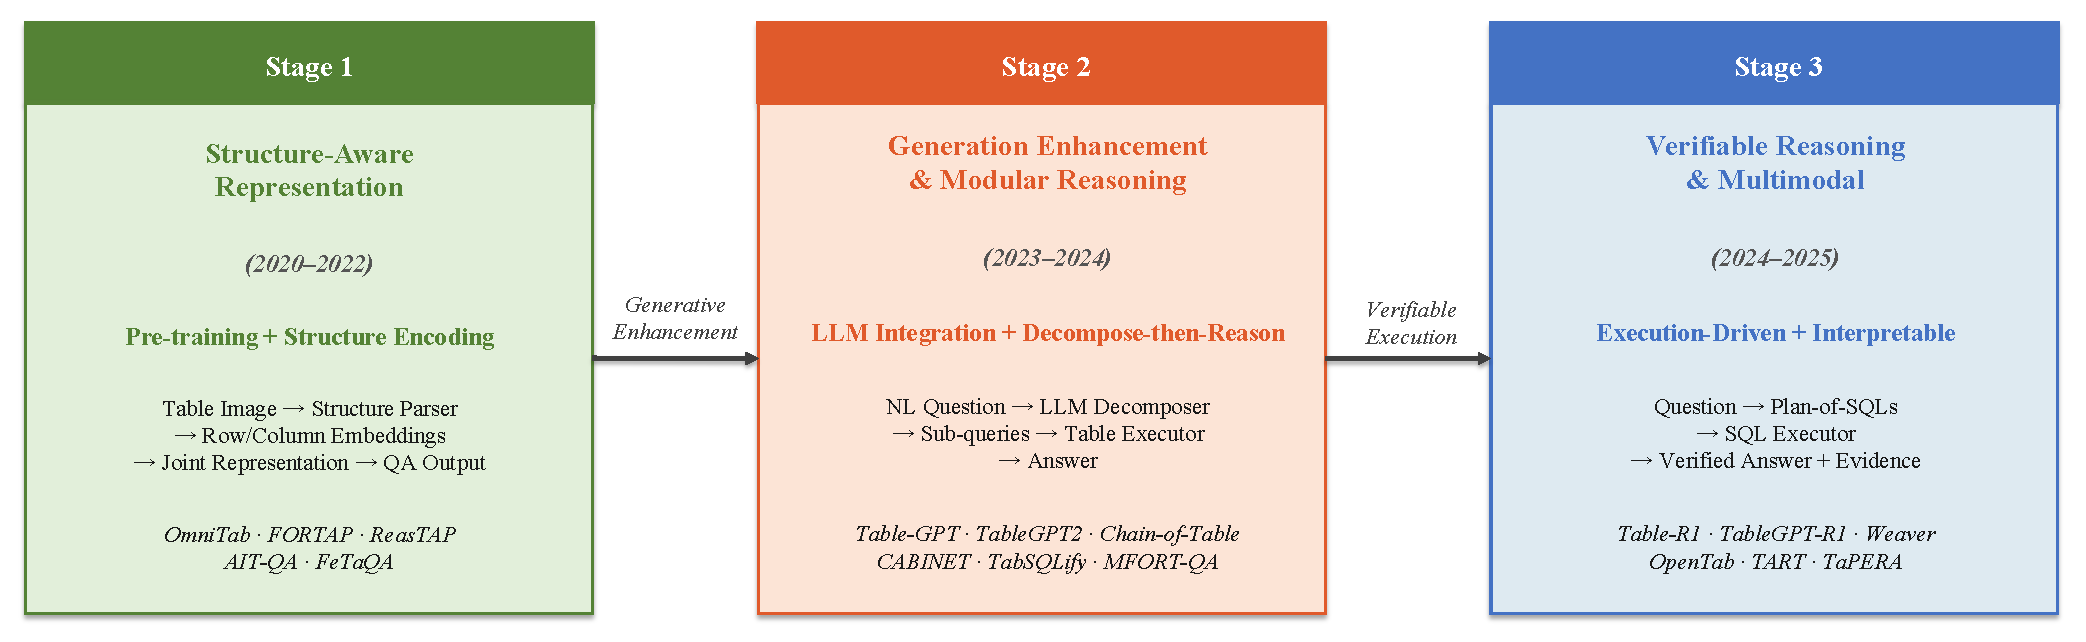
\includegraphics[
    width=0.95\textwidth,
    trim=0cm 0cm 0cm 0cm,
    clip
]{figs_by_qixingyu/fig05.pdf}
\caption{Three-stage evolution of table understanding and question answering (2020--2025): Stage~1 establishes structure-aware representation learning via pre-training and structure encoding; Stage~2 advances generation enhancement and modular reasoning through LLM integration and decompose-then-reason strategies; Stage~3 achieves verifiable reasoning and multimodal understanding driven by execution and interpretable inference.}
\label{fig:table_stages}
\end{figure*}